\chapter{Methodology}
\label{Methodology}

The sample period for the various models we employ is the 250 last daily data points. All calculations are performed every day for all [x] stocks over the whole period used as a rolling window. The period used as a rolling window goes from January 2011 to September 2017, containing about 1500 daily data points. Bear in mind that transaction costs are not incorporated throughout this paper. The methodology of this paper is structured with four main components. 

In the first part of the study we calculate the daily idiosyncratic volatility (IV) for each of the selected stocks by applying the Fama French regression.

Secondly, we pool the stocks into four equally sized, equally weighted portfolios by their constituents proportion of daily IV to daily volatility, which we denote as the daily IV percentage. The equally weighted portfolios are rebalanced daily.

Thirdly, we construct an ARMA-GARCH return forecasting model. We estimate the ARMA-GARCH parameters and construct the one-day-ahead out-of-sample forecasts. Then, we compare the model’s one-day-ahead forecast with the realized return to obtain the daily return forecasting error. This is assigned to its associated portfolio that day and used to revise the return forecasting model. 

Lastly, we revise the return forecasting performance of both the individual stocks and the equally sized, equally weighted portfolios by applying statistical and economical metrics of comparison.

\begin{figure}
\centering
  \centering
  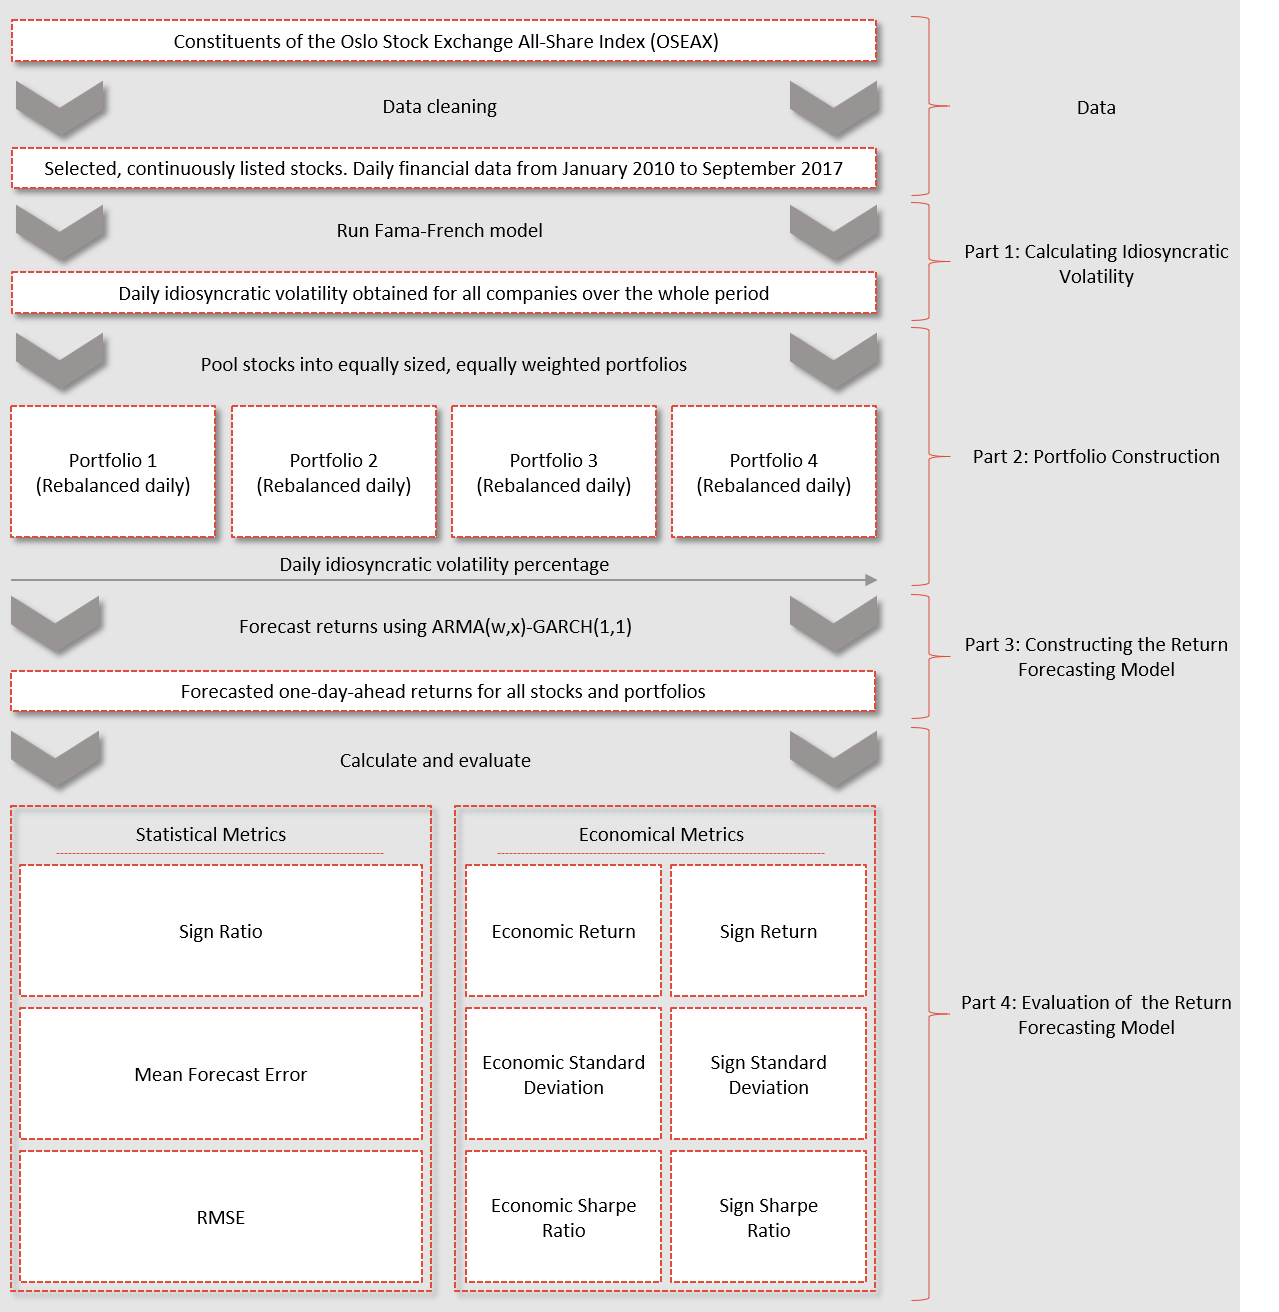
\includegraphics[scale=0.5]{Pictures/FlowChart.png}
  \captionof{figure}{Methodology: Flow Chart}
\end{figure}

\newpage
\section{Calculating the idiosyncratic volatility}

In this section, we describe how we implemented the Fama French three factor model, before we define idiosyncratic volatility.

\subsection{Implementation of the Fama French three factor model} The Fama French three factor model \cite{famafrench} incorporates the empirical fact that value and small-cap stocks have a tendency to outperform the market on a regular basis. Using their methodology we employ the following multiple linear regression:
\begin{align} 
    r_{i,t} - r_{f,t}= \alpha_{i,t} + \beta_{m,i,t}(r_{m,t} - r_{f,t}) + \beta_{SMB,i,t}r_{SMB,t} + \beta_{HML,i,t}r_{HML,t} + \epsilon_{i,t}, \quad  \forall i \in I \quad  \forall t \in T 
    \label{FFregression}
\end{align}

where $t$ indicates the day in the sample period, $r_{i,t}$ is the daily realized return of the stock $i$, $r_{f,t}$ is defined as the daily risk-free rate of Norwegian 10-years government bonds, $r_{m,t}$ is the daily return of the value-weighted market OSEAX portfolio, $r_{SMB,t}$ is the daily excess return of a portfolio consisting of small stocks relative to a portfolio consisting of big stocks, $r_{HML,t}$ is the daily excess return of a portfolio consisting of high book-to-market ratio stocks relative to low book-to-market stocks. $\beta_{m,i,t}$, $\beta_{SMB,i,t}$ and $\beta_{HML,i,t}$ are the corresponding coefficients resulting from the regression and the regression error is $\epsilon_{i,t}$.

More precisely, we define $r_{m,t}$, $r_{HML,t}$ and $r_{SMB,t}$ as:
\begin{align}
    r_{m,t} &= \sum_{i=1}^{N} r_{i,t} \cdot \frac{\text{MC}_{i,t}}{\sum_{s=1}^{N} MC_{s,t}},  \quad  \forall t \in T \\
    r_{SMB,t} &= \sum_{i=1}^{\frac{N}{2}} r_{i,t} \cdot \frac{\text{MC}_{i,t}}{\sum_{s=1}^{\frac{N}{2}} MC_{s,t}} - \sum_{k=\frac{N}{2}+1}^{N} r_{k,t} \cdot \frac{\text{MC}_{k,t}}{\sum_{s={\frac{N}{2}+1}}^{N} MC_{s,t}}, \quad  \forall t \in T \\
    r_{HML,t} &= \sum_{i=1}^{\frac{N}{2}} r_{i,t} \cdot \frac{\text{MC}_{i,t}}{\sum_{s=1}^{\frac{N}{2}} MC_{s,t}} - \sum_{k=\frac{N}{2}+1}^{N} r_{k,t} \cdot \frac{\text{MC}_{k,t}}{\sum_{s=\frac{N}{2}+1}^{N} MC_{s,t}} \quad  \forall t \in T
\end{align}
where $N$ is the number of stocks in the sample, $r_{i,t}$ and $MC_{i,t}$ is the realized return and market capitalization of stock $i$ at day $t$, respectively. 

\subsection{Definition of idiosyncratic volatility}
Consistent with Ang et al. \cite{angetal06} we define idiosyncratic volatility as the square root of the variance of the error term in the Fama French three factor model \cite{famafrench}. Hence, deriving from equation \ref{FFregression}, we have:
 \begin{align}
 IV_{i,t} &= \sqrt{Var[\epsilon_{i,t}]} \\
  &= \sqrt{Var[r_{i,t} - r_{f,t}- \alpha_{i,t}-\beta_{m,i,t}(r_{m,t} - r_{f,t}) - \beta_{SMB,i,t}r_{SMB,t} - \beta_{HML,i,t}r_{HML,t}]},  \quad  \forall i \in I \quad  \forall t \in T \\
 &= \sqrt{Var[r_{i,t}]+\beta_{1,i,t}^2Var[r_{m,t}]+\beta_{SMB,i,t}^2Var[r_{SMB,t}]+\beta_{HML,i,t}^2Var[r_{HML,t}]}, \quad  \forall i \in I \quad  \forall t \in T \\ 
 &= \sqrt{\sigma_{i,t}^2 - \beta^2_{m,i,t} \sigma_{m,t}^{2}- \beta^2_{SMB,i,t} \sigma_{SMB,t}^{2}- \beta^2_{HML,i,t} \sigma_{HML,t}^{2}}, \quad  \forall i \in I \quad  \forall t \in T
 \end{align}
where $t$ is the current day, T is the number of days the rolling window runs over and $IV_{i,t}$ is the IV of stock $i$ in day $t$. 

\section{Portfolio construction pooled by the constituents' daily IV percentage}
We have now described the methodology of estimating the daily IV percentage values. In this study, we seek to examine the relationship between the proportion of a stock's idiosyncratic volatility to volatility, the IV percentage. This because we find it interesting to examine stocks where the IV constitutes a large or small component of the stock's volatility, and not just in terms of magnitude. We define the daily IV percentage as the ratio:
\begin{align}
    \frac{IV_{i,t}}{\sigma_{i,t}}, \quad  \forall i \in I \quad  \forall t \in T
\end{align}

Further, we construct four equally sized, equally weighted portfolios by pooling stocks by their daily IV percentage. Portfolio 1 contains stocks with the lowest daily IV percentage, while portfolio 4 contains stocks with the lowest daily IV percentage. The portfolios are held for one day and the the equally-weighted return at the end of the current day is calculated. We rebalance the portfolios every day. 


\section{Constructing the return forecasting model: a dynamic ARMA($w,x$)-GARCH($1,1$)} 


\subsection{Theoretical background for the ARMA-GARCH return forecasting model}

Financial returns are often modelled as auto-regressive moving average (ARMA) time series with random disturbances having conditional heteroscedastic variances. The conditional mean and conditional variance will change at every point in time because it depends on the history of returns up to that point. That is, we account for the dynamic properties of returns by regarding their distribution at any point in time as being conditional on all the information up to that point. The distribution of a return at time t regards all the past returns up to and including time $t-1$ as being non-stochastic. We denote the information set, which is the set containing all the past returns up to and including time $t-1$, by $I_{t-1}$. The information set contains all the prices and returns that we can observe, like the filtration set in continuous time. 

We write $\sigma_t^2$ to denote the conditional variance at time $t$. This is the variance at time $t$, conditional on the information set. That is, we assume that everything in the information set is not random because we have an observation on it. When the conditional distributions of returns at every point in time are all normal we write:
\begin{align}
    r_t | I_{t-1} \sim N(0,{\sigma_t^2})
\end{align}

Often one would choose other distributions due to the fact that financial series often have fat tails. One option would be to use the Student-t distribution distribution or a skewed version of it. This paper assumes that returns are having a normal distribution. 

\subsubsection{The Conditional Mean Equation, ARMA($w$,$x$)}

For modeling data series we used two common concepts of conditional mean: the auto regressive (AR) process and the moving average (MA) process. Together the two processes constitute the conditional mean equation. 

The AR process is given by:
\begin{align}
    r_{i,t}=c_i + \sum_{j=1}^w\kappa_j r_{i,t-j} + \epsilon_{i,t},\quad \epsilon_{i,t} | I_{i,t-1} \sim N(0,{\sigma_{i,t}^2}) \label{ConditionalMeanEquation}
\end{align}
where $\kappa_j$ is the lag parameter of the observed variable, $r_t$ is the random observed variable at time $t$ dending on the previously realized values of $r_{t-j}$, $c$ is the mean constant and $\epsilon_t$ the white noise.

The MA process is given by:
\begin{align}
    r_{i,t}=c_i + \sum_{j=1}^x\mu_{i,j} \epsilon_{i,t-j} + \epsilon_{i,t},\quad \epsilon_{i,t} | I_{i,t-1} \sim N(0,{\sigma_{i,t}^2}) \label{ConditionalMeanEquation}
\end{align}
where $\mu_j$ is the lag parameter of the observed variable, $r_t$ is the random observed variable at time $t$ depending on the previously realized values of $\epsilon_{t-j}$, $c$ is the mean constant and $\epsilon_t$ the white noise.

The combination of both the AR-process and MA-process, gives us the ARMA process described by:
\begin{align}
    r_{i,t}=c_i+\sum_{j=1}^w\kappa_{i,j} r_{i,t-j}+\sum_{j=1}^x\mu_{i,j} \epsilon_{i,t-j}+\epsilon_{i,t},\quad \epsilon_{i,t} | I_{i,t-1} \sim N(0,{\sigma_{i,t}^2}) \label{ConditionalMeanEquation}
\end{align}

\subsubsection{The Conditional Variance Equation, GARCH($y,z$)}
As financial data time series usually exhibit volatility clustering, a model dealing with
conditional heteroskedasticity should be considered. We use the GARCH model introduced by (Bollerslev, 1986),which is a generalization of the ARCH model that was originally developed by (Engle, 1982). The ARCH model allows for long lags in conditional variance and the GARCH model extends it in the way that it allows for both long lags in conditional variance and a more flexible lag structure.

The GARCH($y$,$z$) has the conditional volatility equation given by:

\begin{align}
    \sigma_{i,t^2} &= \omega_i + \sum_{j=1}^y\alpha_{i,j}\epsilon_{i,t-j}^2+\sum_{j=1}^z\beta_{i,j}\sigma_{i,t-j}^2,\quad\epsilon_{i,t} | I_{i,t-1} \sim N(0,{\sigma_{i,t}^2}) \label{ConditionalVolatilityEquation}
\end{align}

The GARCH error parameter $\alpha$ measures the reaction of conditional volatility to market shocks. When $\alpha$ is relatively large, above 0.1, the volatility is very sensitive to market events.

The GARCH lag parameter $\beta$ measures the persistence in conditional volatility irrespective of anything happening in the market. When $\beta$ is relatively large, above 0.9, then volatility takes a long time to die out.

\subsubsection{Long term volatility}

In the absence of market shocks the GARCH variance will eventually settle down to a steady state value. This is the value $\bar{\sigma}^2$ such that ${\sigma_t^2} = \bar{\sigma}^2$ for all t. We call $\bar{\sigma}^2$ the unconditional variance of the GARCH model. It corresponds to a long term average value of the conditional variance. The theoretical value of the GARCH long term or unconditional variance is not the same as the unconditional variance in a moving average volatility model. The moving average unconditional variance is called the i.i.d. variance because it is based on the i.i.d. returns assumption. The theoretical value of the unconditional variance in a GARCH model is clearly not based on the i.i.d. returns assumption. In fact, the GARCH unconditional variance differs depending on the GARCH model. The long term or unconditional variance is found by substituting ${\sigma_t^2} = {\sigma_{t-1}^2} = \bar{\sigma}^2$ into the GARCH conditional variance equation.We also use the fact that $E(\epsilon_{t-1}^2)=\sigma_{t-1}^2$. This yields the following formula for the long term variance of the GARCH model:

\begin{align}
    \bar{\sigma}_i^2=\frac{\omega_i}{1-(\sum_{j=1}^y\alpha_{i,j}+\sum_{j=1}^z\beta_{i,j})} \label{longTermVolatilityGARCH}
\end{align}

\subsubsection{Parameter Estimation}

The plain vanilla ARMA and ARMA-GARCH parameters are estimated by maximizing the value of the log likelihood function. As mentioned earlier, in this paper we assume that the distribution of the error process is normal with expectation 0 and conditional variance ${\sigma_t^2}$. Furthermore, we have assumed stationarity, so the unconditional variance, in the case of plain vanilla ARMA, is ${\bar\sigma^2}$. With these assumptions in mind, we can use the normal log likelihood function.

\subsubsection{Plain Vanilla ARMA($w,x$)}

Maximizing the ARMA likelihood reduces to the problem of maximizing:
\begin{align} 
    ln(L_{i,t})=-\frac{1}{2}\sum_{t=1}^T\bigg( ln(\sigma_{i}^2)+(\frac{\epsilon_{i,t}}{\sigma_i})^2\bigg)  \label{MaximumLikeARMA}
\end{align}
with respect to all the parameters. To do this we solve the conditional mean equation (\ref{ConditionalMeanEquationARMA}) for $\epsilon_t$:
\begin{align}
     \epsilon_{i,t}=r_{i,t}-\sum_{j=1}^w\kappa_{i,j} r_{i,t-j}-\sum_{j=1}^x\mu_{i,j} \epsilon_{i,t-j}-c_i \label{ConditionalMeanEquationOnEpsilon}
\end{align}
Finally we insert the above equation (\ref{ConditionalMeanEquationOnEpsilonARMA}) and the conditional volatility equation (\ref{ConditionalVolatilityEquation}) into the maximum likelihood function (\ref{MaximumLikeARMA}):
\begin{align} 
    ln(L_{i,t})=-\frac{1}{2}\sum_{t=1}^T\Bigg( ln(\sigma_i^2)+\Big(\frac{(r_{i,t}-\sum_{j=1}^w\kappa_{i,j} r_{i,t-j}-\sum_{j=1}^x\mu_{i,j} \epsilon_{i,t-j}-c_i)^2}{\sigma_i^2}\Big)\Bigg)  \label{fullMaximumLikeARMA}
\end{align}

\subsubsection{ARMA($w,x$)-GARCH($y,z$)}
Maximizing the ARMA-GARCH likelihood reduces to the problem of maximizing:
\begin{align} 
    ln(L_{i,t})=-\frac{1}{2}\sum_{t=1}^T\bigg( ln(\sigma_{i,t}^2)+(\frac{\epsilon_{i,t}}{\sigma_{i,t}})^2\bigg)   \label{MaximumLike}
\end{align}
with respect to all the parameters. The conditional mean equation is solved on epsilon, just as in equation \ref{ConditionalMeanEquationOnEpsilon}. The equation is then inserted, together with the conditional volatility equation (\ref{ConditionalVolatilityEquation}), into the maximum likelihood function (\ref{MaximumLike}):
\begin{align} 
    ln(L_{i,t})=-\frac{1}{2}\sum_{t=1}^T \Bigg(ln\Big(\omega_i + \sum_{j=1}^y\alpha_{i,j}\epsilon_{i,t-j}^2+\sum_{j=1}^z\beta_{i,j}\sigma_{i,t-j}^2\big)+\Big(\frac{(r_{i,t}-\sum_{j=1}^w\kappa_{i,j} r_{i,t-j}-\sum_{j=1}^x\mu_{i,j} \epsilon_{i,t-j}-c_i)^2}{\omega_i + \sum_{j=1}^y \alpha_{i,j} \epsilon_{i,t-j}^2 +\sum_{j=1}^z\beta_{i,j}\sigma_{i,t-j}^2}\Big)\Bigg)   \label{fullMaximumLike}
\end{align}
The parameter constraints are:
\begin{align} 
    \omega_i>0,\quad\quad \alpha_{i,j},\beta_{i,j}\geq0 \quad \forall j, \quad \sum_{j=1}^y\alpha_{i,j}+\sum_{j=1}^z\beta_{i,j}<1 \label{ParameterConstraints}
\end{align}

\subsection{Implementation of the dynamic ARMA($w,x$)-GARCH($1,1$)}
To forecast returns we will try to fit an auto regressive moving average return model (ARMA) of order ($w,x$) with asymmetric generalized auto-regressive conditional hetereoscadasticity (GARCH) of order ($1$,$1$). The estimation of the ARMA($w,x$)-GARCH($1,1$) parameters is done in R, while the rest of the calculations in this paper is done in Python. The reason we chose to calculate the parameters of the ARMA($w,x$)-GARCH($1,1$) in R, is because there are currently no packages in Python supporting ARMA-GARCH, only AR-GARCH. 

The first thing to be decided, is the ARMA order. In other words, we have to decide which values the parameters, $w$ and $x$, in the conditional mean equation (\ref{ConditionalMeanEquation}) should have. The parameters and hence the maximum likelihood is calculated for all combinations of $w$ and $x$, using equation \ref{fullMaximumLikeARMA}, where $w\in[0,3]$ and $x\in[0,3]$. The final values of $w$ and $x$, the ARMA order, to use in our forecast is chosen based on the the Akaike information criterion (AIC). AIC is an estimator of the relative quality of statistical models for a given set of data. Given a collection of models for the data, AIC estimates the quality of each model, relative to each of the other models. Thus, AIC provides a means for model selection. The AIC of a given model is calculated using the following equation:
\begin{align}
    AIC_{i,t}=2k_i-2ln(L_{i,t})
\end{align}
where $k$ is the number of estmated parameters and $L$ is the maximum value of the likelihood function. 

After the decision is made of which ARMA order to use, equation (\ref{fullMaximumLike}) is solved. There is no guarantee that the maximum likelihood of the ARMA-GARCH will converge. To increase the probability of convergence, the algorithm in R tries four different solvers. If there is no convergence, the conditional mean parameters are found using plain vanilla ARMA (\ref{fullMaximumLikeARMA}) and not ARMA-GARCH (\ref{fullMaximumLike}). The maximum likelihood function of plain vanilla ARMA will almost always converge because it is linear. If the plain vanilla ARMA does not converge, the process above is repeated with the ARMA order giving second best AIC, and so on, until convergence is achieved.

The ARMA($w,x$)-GARCH($1,1$) parameters are estimated based on the information set for each stock, $i$, for every time step, over the whole period used as a rolling window. The time step is one-day-ahead and the information set, sample, which the parameters are estimated from are the past 250 daily returns. As mentioned in the introduction to this chapter, there are [x] stocks, the period used as a rolling window is from January 2011 to September 2017, constituting about 1500 trading days. The model setup results in a huge number of needed calculations, and as a consequence, we were granted access to the calculation cluster Solstorm belonging to the Department of Industrial Economics and Technology Management at NTNU. 

One may argue that a information set bigger than 250 should be used, as the standard errors of the parameters are only valid asymptotically. This, additional return forecasting model spesification and other return forecasting models are further discussed in Chapter \ref{FutureWork}.


\subsection{Return forecasting}

After the model in the previous subsection is run on the data, we obtain optimal values for all the parameters for each stock every day. To forecast the the one-day-ahead return, and hence test our out-of sample performance, we need to compute the conditional expected return of the conditional mean equation (\ref{ConditionalMeanEquation}). The expected return at time $t$ for a given stock, $i$, is:
\begin{align} 
    E(r_{i,t})=c_i+\sum_{j=1}^w\kappa_{i,j} r_{i,t-j}+\sum_{j=1}^w\mu_{i,j} \epsilon_{i,t-j} \label{ExpectedConditionalMean}
\end{align}
The expectation of the error process, $\epsilon_t$, is assumed to be zero. The parameters obtained in the previous subsection is our best guess on what the parameters would be tomorrow. Hence, the optimal parameters at time $t$ is used to forecast the return at time $t+1$. Using equation \label{ExpectedConditionalMean}, our forecast at time $t$ for time $t+1$ for a given stock,$i$, is:
\begin{align} 
    E(r_{i,t+1})=c_i+\sum_{j=0}^w\kappa_{i,j} r_{i,t-j}+\sum_{j=0}^x\mu_{i,j} \epsilon_{i,t-j}
\end{align}

\section{Evaluation of the return forecasting model performance}
In the last section we specified the return forecasting model, we now wish to evaluate the model's return forecasting performance in terms of both statistical and economical metrics. 

\subsection{Statistical Metrics}

The return forecasting model produces a series of return forecasting estimates, we calculate the return forecasting error for each day in the out-of-sample period. We define the return forecasting error as:
\begin{align}
    \epsilon_{i,t}^{f} = r_{i,t}^{r} - r_{i,t}^{e}
\end{align}
where $\epsilon_{i,t}^{f}$ is the return forecasting error, the difference between the return forecasting estimate, $r_{i,t}^{e}$, and realized returns, $r_{i,t}^{r}$, for all stocks and all time steps.

In order to assess the return forecasting accuracy and precision, we define two statistical metrics.

Firstly, as a statistical measure of accuracy, we define the mean forecast error, that is the \textbf{bla bla bla}, as:

\textbf{Fyll inn matematisk formel}

Secondly, as a statistical measure of precision, we define the root mean square error metric (RMSE), that is the standard deviation of the residuals, as:
\begin{align}
    RMSE_{\tau} = \sqrt{\frac{\sum_{i=1}^{N}(r_{i,t}^{r} - r_{i,t}^{e})^{2}}{n}}, \quad \forall \tau in \Sigma
\end{align}
where $i$ is stock and $\tau$ is the current period and $\Sigma$ is the total number of periods. We calculate the RMSE for each portfolio and each period, summing the total RMSE for each portfolio over the total sample period, before finding the average by dividing by number for periods:
\begin{align}
    RMSE_{b} = \frac{1}{|\Sigma|}\sum_{\tau=1}^{|\Sigma|}\sqrt{\frac{\sum_{i=1}^{N}(r_{i,t}^{r} - r_{i,t}^{e})^{2}}{n}}, \quad \forall b \in B
\end{align}

Another statistical metric, as a measure of the market timing ability of the return forecasting model, we calculate the proportion of times the model correctly predicted the direction of the return. We define this percentage as Sign and its corresponding return as $r_{sign}$. 

\subsection{Economical Metrics}

Moreover, we also wish to apply economical metrics. 

We define the economic return, $r_{economic}$, as the annualized return obtained from following a buy-and-hold strategy, holding a stock from the start until the end of the period.

Furthermore, we wish to examine the profitability of following the predictions of our return forecasting model, compared to an ordinary buy-and-hold strategy. 

Hence, we define the sign return as following the one-day-ahead predictions from the return forecasting model from the start to the end of the period used as a rolling window. That means taking a long position if the model predicts a positive return, and a short position if the model predicts a negative return for the next day. The annualized return of this strategy is defined as the sign return, $r_{sign}$. If the prediction is correct, the realized return is assigned to the $r_{sign}$. Likewise, if the prediction is wrong, the realized return is withdrawn from the accumulated return, $r_{sign}$.

In addition, we calculate standard deviations of the economic and sign return. We define alpha, $\alpha$, as the difference $r_{sign}-r_{economic}$. This is the excess return from following the sign strategy compared to the buy-and-hold strategy. 

Finally, we find the Sharpe ratio of the annualized economic return and annualized sign return, respectively. The Sharpe ratio is defined as the excess return over the risk free rate, divided by the standard deviation.
